\section{Methodology}

%%%%%%%%%%%%%%%%%%%%%%%%%%%%%%%%
% Preliminaries
%%%%%%%%%%%%%%%%%%%%%%%%%%%%%%%%

\subsection{Preliminaries}

\subsubsection{Problem Formulations}

\paragraph{Markov Decision Processes}

In RL, problems are typically formulated as a Markov decision process (MDP) \cite{sutton1998reinforcement}.
An MDP is defined as a tuple $\langle S, A, P, R, \gamma \rangle$, where $S$ and $A$ denote the state and action spaces, $P$ is the transition probability, $R$ is the reward function, and $\gamma \in [0, 1)$ is the discount factor.
The objective of RL is to find an optimal policy $\pi^*$ that maximizes the cumulative reward, defined as:
\begin{equation} \label{eq:mdp_optimization_problem}
    \begin{aligned}
        J_R(\pi) &= \mathbb{E}_{\tau \sim \pi}\!\left[\sum^\infty_{t = 0} \gamma^t R(s_t, a_t)\right] \\
        \pi^* &= \arg \max J_R(\pi)
    \end{aligned}
\end{equation}
Here, $\tau = (s_0, a_0, s_1, a_1, \ldots)$ denotes a trajectory generated by following policy $\pi$.

\paragraph{Constrained Markov Decision Processes}

In contrast, constrained RL is typically formulated as a constrained Markov decision process (CMDP) \cite{altman2021constrained}. A CMDP extends an MDP by introducing a set of cost functions $C_1, \ldots, C_m$, which are separate from the reward function, together with corresponding limits $d_1, \ldots, d_m$.
Formally, a CMDP is defined as a tuple $\langle S, A, P, R, C, d, \gamma \rangle$.
In a CMDP, the set of feasible policies $\Pi_C$ is defined as:
\begin{equation} \label{eq:feasible_policy_set_cmdp}
    \begin{aligned}
        \Pi_C = \{ \pi \in \Pi: \forall i, J_{C_i}(\pi) \leq d_i \},
    \end{aligned}
\end{equation}
Specifically, the constraint function for constraint $i$ is defined as the expected cumulative discounted cost:
\begin{equation} \label{eq:cost_return}
    J_{C_i}(\pi) = \mathbb{E}_{\tau \sim \pi}\!\left[\sum^\infty_{t = 0} \gamma^t C_i(s_t, a_t)\right], 
    \quad \forall i \in \{1, \ldots, m\}.
\end{equation}
In standard RL, the objective is an unconstrained policy optimization problem that aims to find a policy maximizing the expected return, as defined in Eq.~\eqref{eq:mdp_optimization_problem}.
Whereas constrained RL solves a policy optimization problem that maximizes the expected return subject to the cost constraints defined in Eq.~\eqref{eq:cost_return}.
\begin{equation} \label{eq:cmdp_optimization_problem}
    \pi^* = \arg\max_\pi J_R(\pi) \; \text{s. t.} \; J_{C_i}(\pi) \leq d_i, \; \forall i \in {1, \ldots, m}.
\end{equation}


\paragraph{State-wise Constrained Markov Decision Process}

The CMDP framework can be extended to use various types of cost-based constraints.
One such extension is the state-wise constrained Markov decision process (SCMDP) \cite{zhao2023state}, which imposes state-wise constraints to bound the expected cost at each state by a specified threshold.
In a SCMDP, the set of feasible policies $\Pi_{SC}$ is defined as:
\begin{equation} \label{eq:feasible_policy_set_scmdp}
    \begin{aligned}    
        \Pi_{SC} = \{ \pi \in \Pi: &\; \forall (s_t, a_t, s_{t + 1}) \sim \tau, \\
                                &\; \forall i, C_i(s_t, a_t, s_{t + 1}) \leq w_i \}
    \end{aligned}
\end{equation}
where $C_i(s_t, a_t, s_{t + 1})$ is the cost incurred at state $s_t$ after taking action $a_t$ and transitioning to state $s_{t + 1}$, and $w_i$ is the corresponding limit.
Similar to CMDP, the optimization problem in SCMDP can be formulated as
\begin{equation} \label{eq:scmdp_optimization_problem}
    \pi^* = \arg\max_\pi J_R(\pi) \; \text{s.t.} \; J_{SC_i}(\pi) \leq w, \; \forall i \in 1, \ldots, m
\end{equation}  % refrence: https://arxiv.org/pdf/2306.12594
In this formulation, the state-wise constraint is defined as:
\begin{equation} \label{eq:statewise_cost_return}
    J_{SC_i}(\pi) = \mathbb{E}_{(s_t, a_t, s_{t + 1}) \sim \tau, \, \tau \sim \pi} \big[ C_i(s_t, a_t, s_{t + 1}) \big], 
    \quad \forall i \in \{1, \ldots, m\}.
\end{equation}
In the CMDP, constraints are imposed only on the cumulative cost, whereas the SCMDP enforces them on the state-wise cost, ensuring safety at each state, as shown in Fig.~\ref{fig:constrained_rl_vs_statewise_constrained_rl}.
% TODO: cost 계산만 다르게 할거면 그림은 통일
% TODO: 그림 quality가 낮음
% TODO: caption의 설명을 어디서 할건지? 지금까지 설명한 내용으로 충분하지 않은가요?
\begin{figure}[H]
    \centering

    % (a) Constrained RL
    \begin{subfigure}{0.46\textwidth}
        \centering
        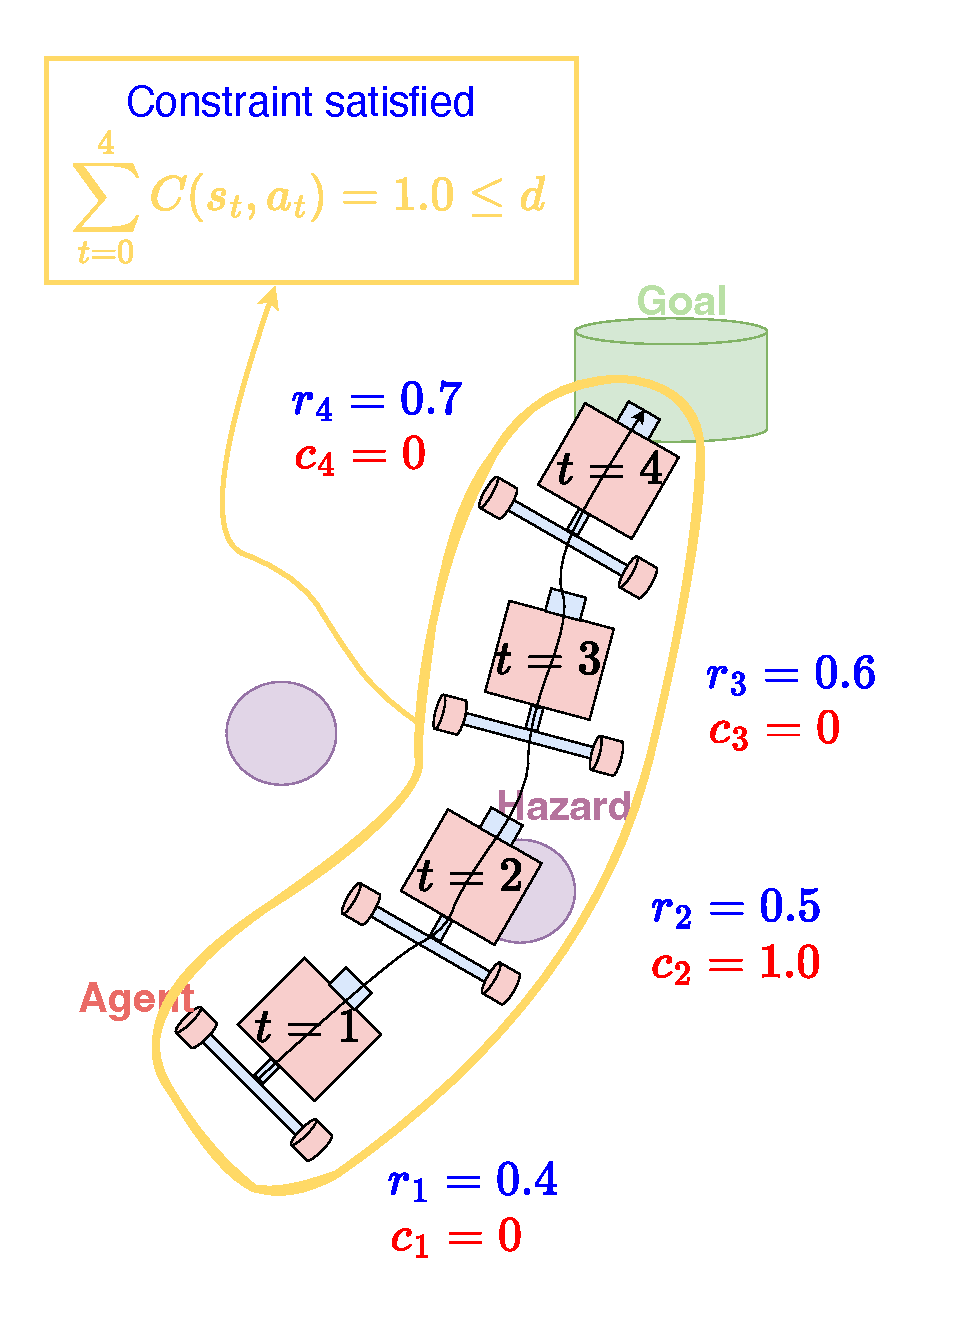
\includegraphics[width=\linewidth]{figure/constrained-rl.pdf}
        \caption{Constrained RL}
    \end{subfigure}
    \hfill
    % (b) State-wise constrained RL
    \begin{subfigure}{0.48\textwidth}
        \centering
        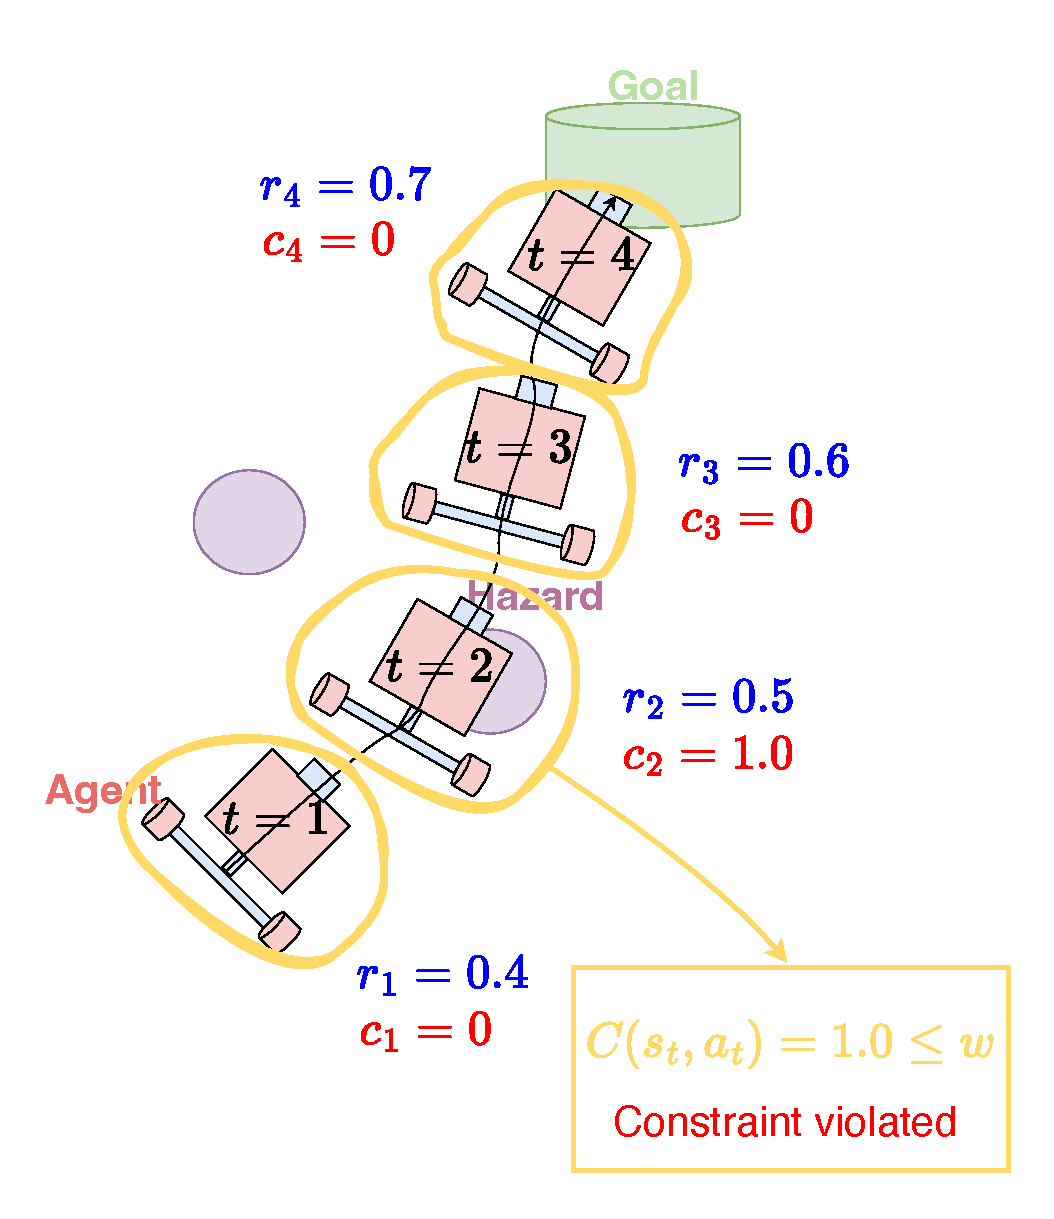
\includegraphics[width=\linewidth]{figure/statewise-constrained-rl.pdf}
        \caption{State-wise constrained RL}
    \end{subfigure}
    \caption{Comparison of constrained RL and state-wise constrained RL.
            In constrained RL, a policy is feasible if the cumulative cost is below the limit.
            In state-wise constrained RL, a policy is feasible if the cost at every state is below the limit.}
    \label{fig:constrained_rl_vs_statewise_constrained_rl}
\end{figure}



\subsubsection{Lagrangian Relaxation for Constrained Policy Optimization} \label{subsubsec:lagrangian_relaxation}

A common approach to solve constrained optimization problems is to use Lagrangian relaxation.
In this approach, the constrained optimization problem \eqref{eq:cmdp_optimization_problem} is reformulated as an unconstrained optimization problem by introducing Lagrange multiplier $\lambda \geq 0$ that penalizes constraint violations.
The resulting Lagrangian can be written as:
\begin{equation}
    L(\theta, \lambda) = J_R(\pi_\theta) - \lambda^\top (J_C(\pi_\theta) - d),
\end{equation}
where $\theta$ denotes the parameter of the policy.
The objective is then to find a saddle point $(\theta^*, \lambda^*)$ that satisfies:
\begin{equation}
    L(\theta^*, \lambda) \geq L(\theta^*, \lambda^*) \geq L(\theta, \lambda^*).
\end{equation}
Since finding a global saddle point is often computationally intractable, in practice one aims to find a locally optimal solution using iterative updates of the policy parameters and the Lagrange multiplier. 
A common approach is to apply gradient-based updates of the form
\begin{align}
    \theta_{n+1} &= \theta_n + \eta_\theta \nabla_\theta \Big(J_R(\pi_\theta) - \lambda_n^\top J_C(\pi_\theta)\Big), \\
    \lambda_{n+1} &= \Big[ \lambda_n + \eta_\lambda \big( J_C(\pi_\theta) - d \big) \Big]_+,
\end{align}
where $\eta_\theta, \eta_\lambda > 0$ are step sizes, and $[\cdot]_+$ denotes the projection onto the nonnegative reals to ensure $\lambda \geq 0$.

%%%%%%%%%%%%%%%%%%%%%%%%%%%%%%%%
% PPO Lagrangian
%%%%%%%%%%%%%%%%%%%%%%%%%%%%%%%%

\subsection{Formulations of PPO under MDP and CMDP}

\paragraph{\textbf{PPO}}

Among policy gradient methods, PPO is one of the most widely used algorithms, proposed to solve the optimization problem in Eq.~\ref{eq:mdp_optimization_problem}.
To improve stability, PPO introduces a clipping mechanism that prevents large policy updates.
The objective function of PPO is defined as:
\begin{equation} \label{eq:ppo_objective}
    J^{\text{PPO}}(\theta) = \mathbb{E}_{\pi_{\theta_\text{old}}} \left[ \min \left( r(\theta) A^{\pi_{\theta_\text{old}}}(s, a), \text{clip}(r(\theta), 1 - \epsilon, 1 + \epsilon) A^{\pi_{\theta_\text{old}}}(s, a) \right) \right]
\end{equation}
where $r(\theta) = \frac{\pi_\theta(a|s)}{\pi_{\theta_\text{old}}(a|s)}$ denotes the probability ratio between the current and the old policies, and $A^{\pi_{\theta_\text{old}}}(s, a) = Q^{\pi_{\theta_\text{old}}}(s, a) - V^{\pi_{\theta_\text{old}}}(s)$ represents the advantage function under the old policy.

\paragraph{\textbf{PPO Lagrangian}}

PPO Lagrangian is proposed as an extension of PPO to the constrained RL setting, enabling the algorithm to handle explicit constraints.
The original PPO algorithm enhances stability by limiting policy updates through clipping, as defined in Eq.~\ref{eq:ppo_objective}, but it does not directly handle constraints.
To address constraints defined in terms of the cumulative cost in Eq.~\ref{eq:cost_return}, PPO Lagrangian applies the Lagrangian relaxation technique, as discussed in Section~\ref{subsubsec:lagrangian_relaxation}, thereby converting the constrained optimization problem in Eq.~\ref{eq:cmdp_optimization_problem} into an unconstrained one.
\begin{equation} \label{eq:ppo_lagrangian_objective}
    \begin{aligned} J^{\text{PPO-Lag}}(\theta)
        = \mathbb{E}_{\pi_{\theta_\text{old}}} \Big[ &\min \big( r(\theta) A^{\pi_{\theta_\text{old}}}(s, a), \text{clip}(r(\theta), 1 - \epsilon, 1 + \epsilon) A^{\pi_{\theta_\text{old}}}(s, a) \big)
        \\ &- \lambda r(\theta) A^{\pi_{\theta_\text{old}}}_c \Big]
    \end{aligned}
\end{equation}
where $\lambda \geq 0$ is the Lagrange multiplier that imposes a penalty on constraint violations.


%%%%%%%%%%%%%%%%%%%%%%%%%%%%%%%%
% Methodology
%%%%%%%%%%%%%%%%%%%%%%%%%%%%%%%%

\subsection{Proposed Method}


% TODO: 이 figure를 쓸거면 본문에서 언급해야 함
% TODO: figure quality가 낮음

\begin{figure}[h]
    \centering

    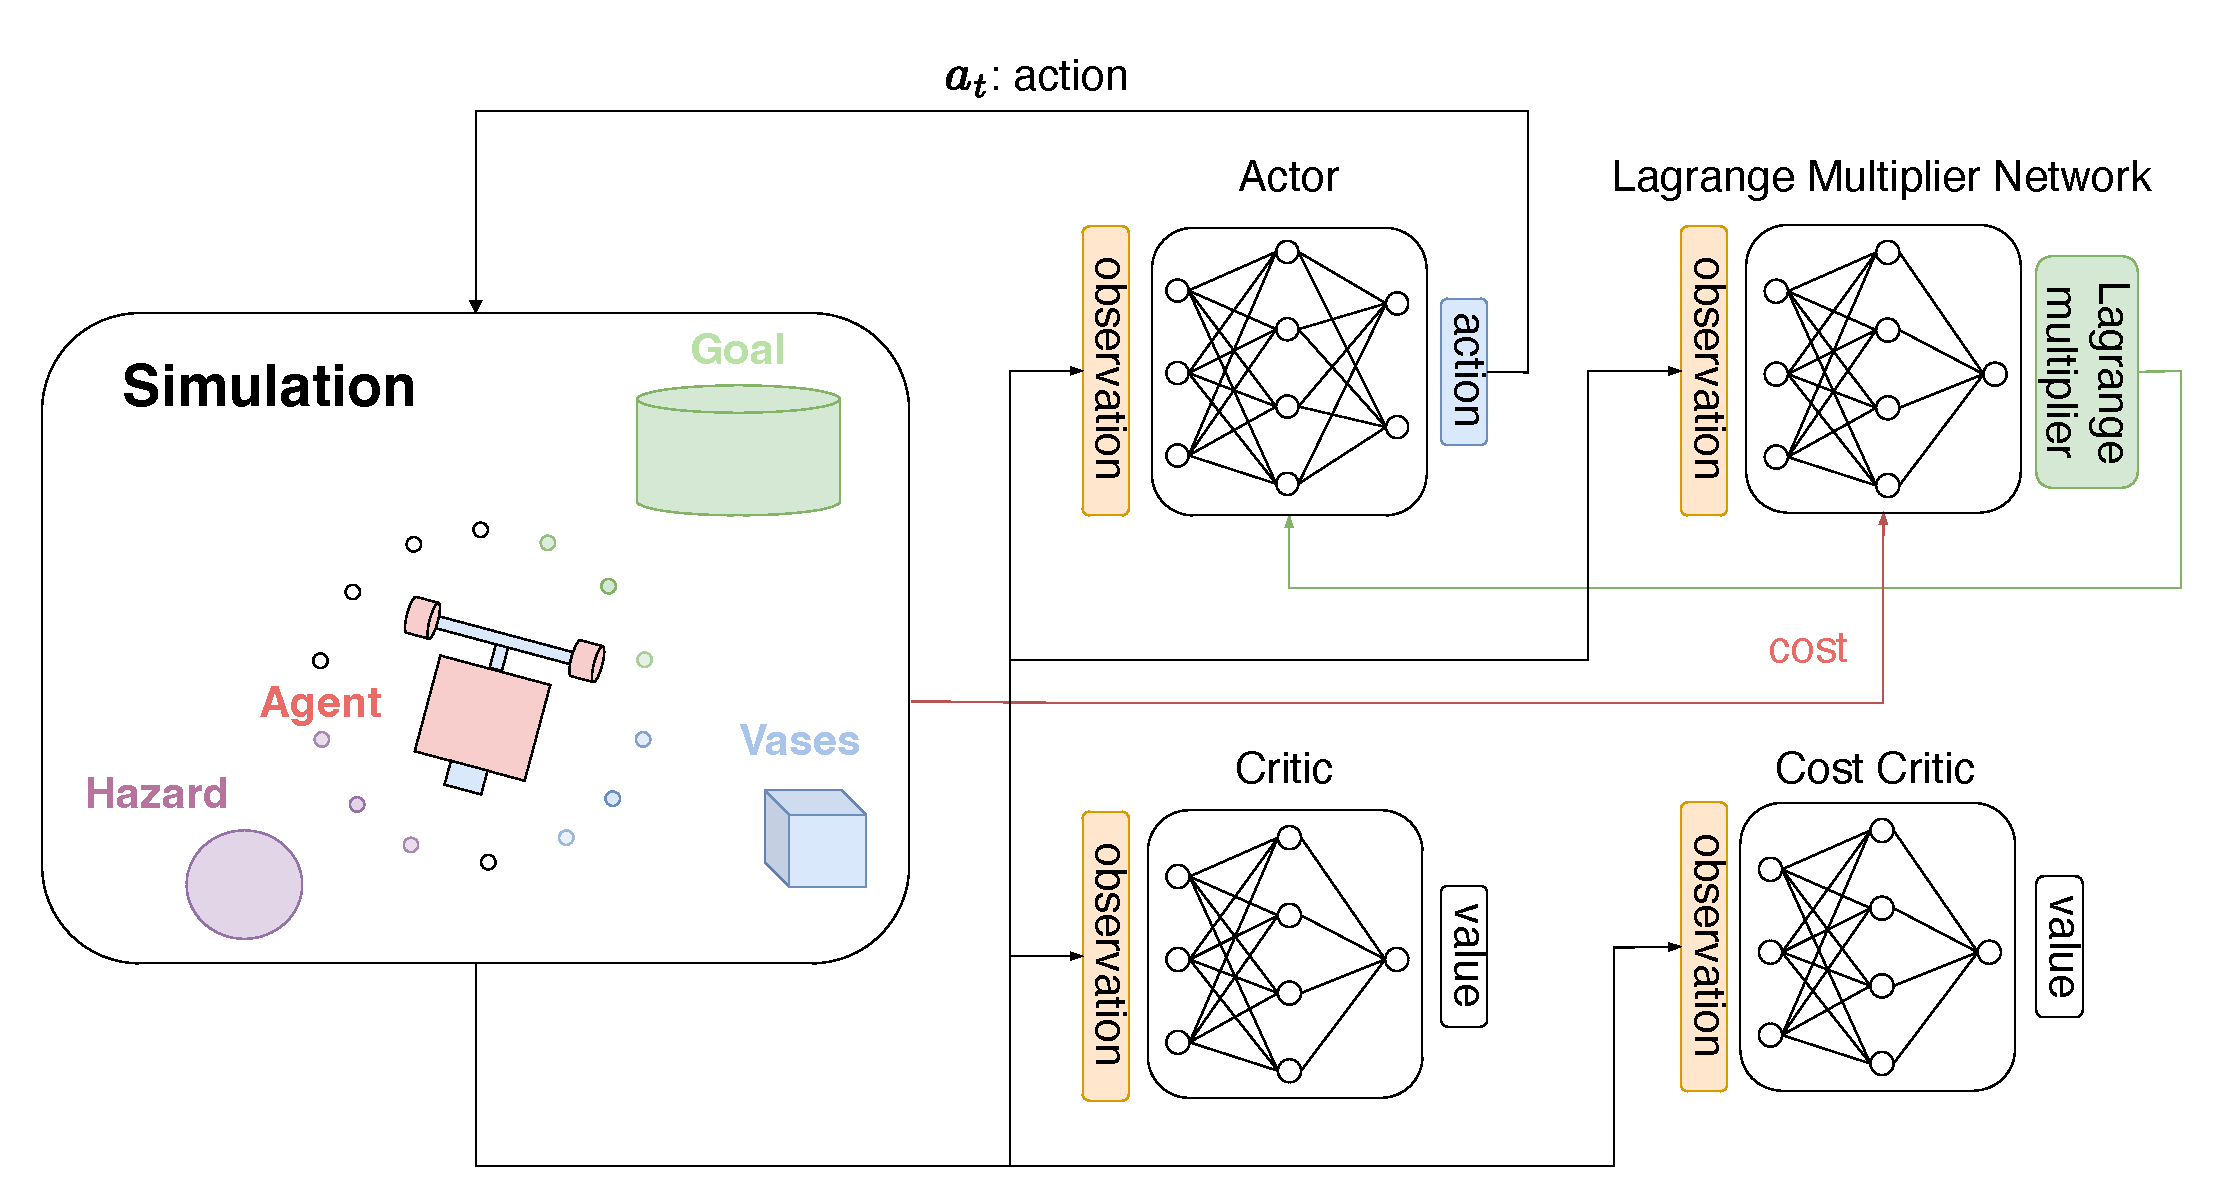
\includegraphics[width=0.8\linewidth]{figure/ppo_lagnet.pdf}
    \caption{Overview of the proposed method.
            Unlike standard PPO-Lagrangian, which employs a scalar Lagrange multiplier due to the constraint being defined on cumulative cost, our approach imposes constraints in a state-wise manner, requiring state-varying multipliers. 
            To estimate these multipliers, we introduce an additional neural network, termed the Lagrange multiplier network.}
    \label{fig:ppo_lagnet}
\end{figure}

% TODO: PPO Lagrangian에 대한 설명이 없음
% TODO: PPO Lagrangian과의 차이를 명확히 언급 (단순히 NN을 썼다고 한 것만으로는 불충분)
In this paper, we propose a method that extends PPO Lagrangian to the state-wise constrained RL setting by estimating state-wise Lagrange multipliers.
Similar to PPO Lagrangian in Eq.~\ref{eq:ppo_lagrangian_objective}, which employs a scalar Lagrange multiplier to handle constraints on the cumulative cost, addressing the state-wise constraint defined in Eq.~\ref{eq:statewise_cost_return} requires a state-varying multiplier.
To this end, we introduce an additional neural network, referred to as the Lagrange multiplier network, which maps a state to its corresponding Lagrange multiplier, as illustrated in Fig.~\ref{fig:ppo_lagnet}.
Formally, the Lagrange multiplier network is parameterized by $\xi$ and is denoted as $\lambda_\xi(s)$.
This allows the application of Lagrangian relaxation to the constrained policy optimization defined in Eq.~\ref{eq:scmdp_optimization_problem}, analogous to the way PPO-Lagrangian handles cumulative cost constraints.
The objective function of the proposed method can thus be expressed as:
\begin{equation} 
    \begin{aligned} J^{\text{Proposed}}(\theta) 
        = \mathbb{E}_{\pi_{\theta_\text{old}}} \Big[ &\min \big( r(\theta) A^{\pi_{\theta_\text{old}}}(s, a), \text{clip}(r(\theta), 1 - \epsilon, 1 + \epsilon) A^{\pi_{\theta_\text{old}}}(s, a) \big) 
        \\ &- \lambda_\xi(s) r(\theta) A^{\pi_{\theta_\text{old}}}_c \Big] 
    \end{aligned} 
\end{equation}
The parameters of the Lagrange multiplier network are updated using the following objective:
\begin{equation} \label{eq:lagrange_multiplier_update}
    J_\lambda(\xi) = \mathbb{E}_{(s_t, a_t, s_{t + 1}) \sim \tau, \tau \sim \pi_{\theta_\text{old}}} [\lambda_\xi(s_t) (C(s_t, a_t, s_{t + 1}) - w)]
\end{equation}
where $w$ denotes the state-wise cost limit. 
In this formulation, the objective $J_\lambda(\xi)$ drives the multiplier $\lambda_\xi(s)$ to increase when the observed cost $C(s_t, a_t, s_{t+1})$ exceeds the limit $w$, and to decrease when it falls below $w$.
